%%%%%%%%%%%%%%%%%%%%%%%%%%%%%%%%%%%%%%%%%%%%%%%%%%%%%%%%%%%%%%%%%%%%%%%%%%%%%%
% Detta är ett exempel på ett latexdokument.
% 
% Alla dokument består av följande delar:
%
%          \documentclass[optioner]{dokumentklass}
%            ...inställningar...
%          \begin{document}
%            ...text...
%          \end{document}
%
% Som ni kanske redan har förstått är används procent (%) för
% kommentarer.
%%%%%%%%%%%%%%%%%%%%%%%%%%%%%%%%%%%%%%%%%%%%%%%%%%%%%%%%%%%%%%%%%%%%%%%%%%%%%%

\documentclass[a4paper]{article}
\bibliographystyle{vancouver}
\usepackage[utf8]{inputenc}
\usepackage[T1]{fontenc}                % För svenska bokstäver
\usepackage[swedish]{babel}             % För svensk avstavning och svenska
\usepackage{graphicx}
\usepackage{url}
\title{Datavetaren Niklaus Emil Wirth}
\author{Lorenz Gerber}
\date{}           % Blir dagens datum om det utelämnas

\begin{document}

\maketitle                      % Skriver ut rubriken som vi
                                % deklarerade ovan med \title, \author
                                % och eventuellt \date

\begin{figure}[ht!]
\centering
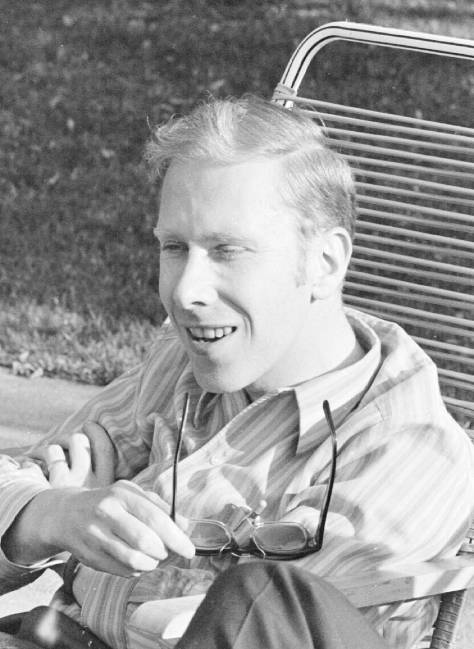
\includegraphics[width=90mm]{Niklaus_Wirth_large.jpg}
\caption{Niklaus Wirth, undated. Source: www.wikipedia.com (GNU Free
  Documenation License 1.2) \label{portrait}}
\end{figure}

\section{Introduktion}          % Detta kommando gör en rubrik

Niklaus E. Wirth är en få icke amerikanska datavetare som har vunnit
`Turingpriset', en utmärkelse som är nämnd efter den engelska datavetar 
pionären Allan Turing \cite{TuringAward}. Niklaus Wirth är född och uppvuxen i Schweiz. Han fick 
`Turingpriset' 1984 för att ha utvecklad flera nya, innovativa
programmeringsspråk \cite{WirthAward}.

\section{Utbilding och Karriär}

Winterthur, staden där Niklaus Wirth är född och uppvuxen ligger inte långt bort 
från Zurich där han började studerade elektronik ingejör på den anrika
tekniska högskolan `Eidgenössische Technische Hochschule' (ETH). Efter 
ingenjörsexamen fortsatte Niklaus Wirth till en MSc på Laval Universitet i Kanada. 
Sen doktorerade han i Berkley (University of California). För några år var han  
assistens professor på Stanford Universitet och sedan i Schweiz på Zurich Universitet. 
1968 fick han en professor tjänst i samma institut som han började sin akademisk 
utbildning, ETH Zurich. Han forskade och undervisade där fram till 1999. I
skrivande stund är Niklaus Wirth 81 år gammal.   

\section{Turingpriset}
I motivering till Wirth's Turingpris står det `För utvecklandet av en rad 
innovativa programspråk: EULER, ALGOL-W \cite{ALGOL}, MODULA
\cite{modula} och PASCAL \cite{PASCAL}.' Av de nämnda språk 
är kanske `Pascal' den mest kända \cite{PASCAL}. Den användes flitigt både i utbildningssyfte 
på universiteter men även i produktiva system. Till exempel så var den ursprungliga
operativsystemet till `Macintosh' datorer skriven i Pascal, så som källkoden av
den mäktiga typsättningsspråket \TeX\ från Donald Knuth. 

\subsection{Mjukvarukrisen}
Under 60' talet blev hårdvaran mer och mer kraftfull medan de vertyg och språk som 
användes till programmering hade inte utvecklads i samma utsträckning. Det resulerade
i att färdigställning av stora mjukvaru projekt ofta blev försenad och budgeten
överskreds. Många projekt kunde inte ens realiseras enligt specifikationer 
och mjukvaruns tillförlitlighet såsom underhållbarhet var mycket
dåliga. Genom Wirth's stora bidrag i utvecklingen av programeringsspråk som följde
och definerade den då nyupkommande paradigm av strukturerad programering 
hjälpte han att komma ur mjukvaru krisen \cite{stepwise}.

\subsection{Strukturerad programmering}
Strukturerad programmering var och är Niklaus Wirth's stora
grej. Paradigment kan sammanfattas med de två ord `hierarki' och
`modularitet' \cite{algorithms}. Två egenskaper som är nu självklart i de flesta moderna
programmerings språk. I strukturerad programmering använder man
`toppen-ned-ansats'
för att lösa problemet: Man definerar problement och delar det upp i
mindre delproblem. De i sin tur delar man igen upp i mindre del
problem tills man kommer ner till nivået där man har färdiga standard
lösningar. Genom den strategi skapas det automatiskt modulärt kod
som går att återanvända för likadana problem.

\section{Efter Turingpriset}
Nikolaus Wirth fick Turingpriset när han var 52 år gammal, egentligen
mitt under hans akademiska karriär. Då är det kanske inte så 
förvånanstvärt att det blev även en del uppmärksammade utvecklingar 
under hans senare karriär. En av de är säkert programmerings språket
`Oberon' som han sen också använde för att skriva ett helt
operativsystem med samma namn \cite{oberon}. I ett interview berättar han, att han
ville ha en likandant dator som han använde under hans sabbatical på 
PARC en då revolutionär masking med namnet `Alto'. Så bestämde han sig
helt enkelt att bygga en likadant dator själv. Systemet `Obereon' var
ett exempel på strukturerad, minimalistiskt arkitektur. Den användes
flitigt på ETH, både i beräknings vetenskaper men så klart också i 
utbildnings syfte av nya generationer av datavetare. Efter Niklaus
Wirth gick i pension, så gjorde han i sin fritid en ny version av
`Oberon' systemet där han den gång till och med designade själv
processorn (implementerad på en så kallad `på-plats-programmerbar 
grindmatris'). Hela projekted finns att ladda ner som öppet källkod \cite{oberonDown}. 
 
\bibliography{testbib}
\end{document}                 % The input file ends with this command.
